\chapter{Domain Adaptation in Imitation Learning with DAIL-GAN Agent\label{ch:DAIL}}


\renewcommand{\SectionsDir}{Chapter3/Sections}
\renewcommand{\SubsectionsDir}{Chapter3/Sections/Subsections}
\renewcommand{\FigsDir}{Chapter3/Figs}
\renewcommand{\TablesDir}{Chapter3/Tables}


In this chapter, the \DAIL\ agent is presented in order to address the domain adaptation problem in imitation learning.


\section{Introduction\label{ch:DAIL:sec:Introduction}}
Imitation learning works by extracting information about the behavior of the expert and learning a mapping between the observation state and demonstrated behavior \cite{schaal1999imitation,IL_Survey_RobotLearning}.
Unfortunately,
the traditional imitation learning algorithms are still far from being comparable with the human imitation due to the lack of the following abilities:

\begin{enumerate}
  \item
        Humans tend to imitate the goal of a task rather than a particular behavior of the expert \cite{baker2007goal,bao2017imitation}.
  \item
        Humans can recognize structural differences (i.e., domain shift) and similarities between the expert and themselves in order to adapt their behaviors accordingly \cite{tomov2021multi}.
\end{enumerate}

The first aspect of human imitation can be modeled using Inverse Reinforcement Learning (IRL)~\cite{ng2000algorithms, abbeel2004apprenticeship}.
IRL seeks to estimate a reward function to explain an expert behavior from demonstrations and subsequently train an agent on it \cite{ng2000algorithms,abbeel2004apprenticeship,levine2011nonlinear,ziebart2008maximum}.
Recent studies \cite{IL_Model_GAIL,DAIL_Model_DAIL,pmlr-v70-baram17a,behbahani2019learning,10.5555/3294996.3295138,zhang2020cgail,chi2020collaborative,zhou2020modeling} utilize Generative Adversarial Network (GAN) \cite{GAN_Original}, which has a discriminator to judge whether a given behavior is from an expert or agent, and then a policy is trained using the discriminator as a reward.
However, these approaches do not take into account the second aspect of human learning: imitation with the presence of domain shift between the expert and the agent.
Such domain shift can mislead the feature learning, resulting in poor task performance.


The problem is formalized as domain adaptation in imitation learning,
which is a process of learning how to perform a task optimally in the learner agent domain,
given demonstrations of the task in a distinct expert domain
\cite{DAIL_Model_DAIL}.
In order to solve this problem,
the authors in
\cite{DAIL_Model_DAIL} proposed a two-step approach:
alignment followed by adaptation.
Firstly,
the Generative Adversarial MDP Alignment (GAMA) was introduced to learn the state -- action maps from demonstrations.
Then,
in the adaptation step, an optimal policy for the learner domain was obtained using the learned alignment from the first step.
Despite showing a promising result,
their agent was evaluated only in low-dimensional tasks.
Besides,
they updated the learned policy by using behavioral cloning, which was vulnerable to cascading errors.
This could lead to poor adaptation performance in more complex high-dimensional tasks.

Unlike previous studies, a novel agent, namely \DAIL{}, is proposed that aims to learn both domain-shared and domain-specific features.
Such features enable the agents to learn optimal policies without being affected by the shift between two domains.
The learning procedure can be achieved within one training process by utilizing adversarial learning \cite{GAN_Original}.
It enables the agent to learn the extracted features, while at the same time, seeking for an optimal learner domain policy.
A comprehensive experiment on both low and high-dimensional tasks is conducted to evaluate the performance of the proposed \DAIL{} agent.


\section{Problem Formulation\label{ch:DAIL:sec:ProblemFormulation}}
The domain adaptation in imitation learning can be formalized as a Markov decision problem which was introduced in Chapter~\ref{ch:Background}.
As a brief reminder,
an episodic Markov Decision Process (MDP) $\mathbb{M}$ with finite time horizon $H$ \cite{RL_AnIntroductionBook} is represented as the following equation:

\[
  \mathbb{M} = (\mathcal{S}, \mathcal{A}, P, R, \gamma, H)
\]

where
$\mathcal{S}$ and $\mathcal{A}$
represent the state and action spaces,
respectively;
$P(s'|s, a)$ denotes the transition function,
$R: \mathcal{S} \times \mathcal{A} \to \mathbb{R}$ is the reward function,
$\gamma$ is the discount factor---whereas,
a policy $\pi(s|a): \mathcal{S} \to \mathcal{A}$ for $\mathbb{M}$
describes a mapping from states $\mathcal{S}$ to actions $\mathcal{A}$.

It should be noted that in the domain adaptive imitation learning setting,
the reward function is not given beforehand.
Therefore,
the MDP for a domain $x$ without reward is defined as
$\mathbb{M}^-_x = (\mathcal{S}_x, \mathcal{A}_x, P_x, \gamma_x, H_x)$.
All examined domains are assumed to be alignable.
That is, if considering two domains $x$ and $y$, $\mathbb{M}^-_x$ can be reduced to $\mathbb{M}^-_y$,
denoted as $\mathbb{M}^-_x \ge \mathbb{M}^-_y$, or vice versa \cite{DAIL_Model_DAIL}.
An example is illustrated in Figure \ref{ch:DAIL:fig:MDP_Reduction}.
Based on this expression,
let $\mathcal{E}$ and $\mathcal{L}$ be the expert and the learner (agent) domain,
respectively,
$\mathbb{M}^-_\mathcal{E}$ and $\mathbb{M}^-_\mathcal{L}$ are said to be alignable if and only if $\mathbb{M}^-_\mathcal{E} \ge \mathbb{M}^-_\mathcal{L}$ or $\mathbb{M}^-_\mathcal{L} \ge \mathbb{M}^-_\mathcal{E}$ \cite{DAIL_Model_DAIL}.

Furthermore, $\tau_{x} = \{(s^t_{x}, a^t_{x}) : t \in [0, \mathcal{H}]\}$ denotes a demonstration in the domain $x$,
which is a sequence of state--action pairs.
Then, a set of demonstrations
$\mathcal{D}_\mathcal{E}=\{\tau^i_\mathcal{E} : i\in[1,N]\}$ from $\mathcal{E}$ is assumed to be available at the training time.
With those assumptions,
the main objective is being able to learn an optimal learner domain policy $\pi^{*}_\mathcal{L}$ against unknown reward functions $\mathcal{R}_\mathcal{E}$ and $\mathcal{R}_\mathcal{L}$, given the expert demonstrations $\mathcal{D}_{\mathcal{E}}$.

\begin{figure}[htbp!]
  \centering
  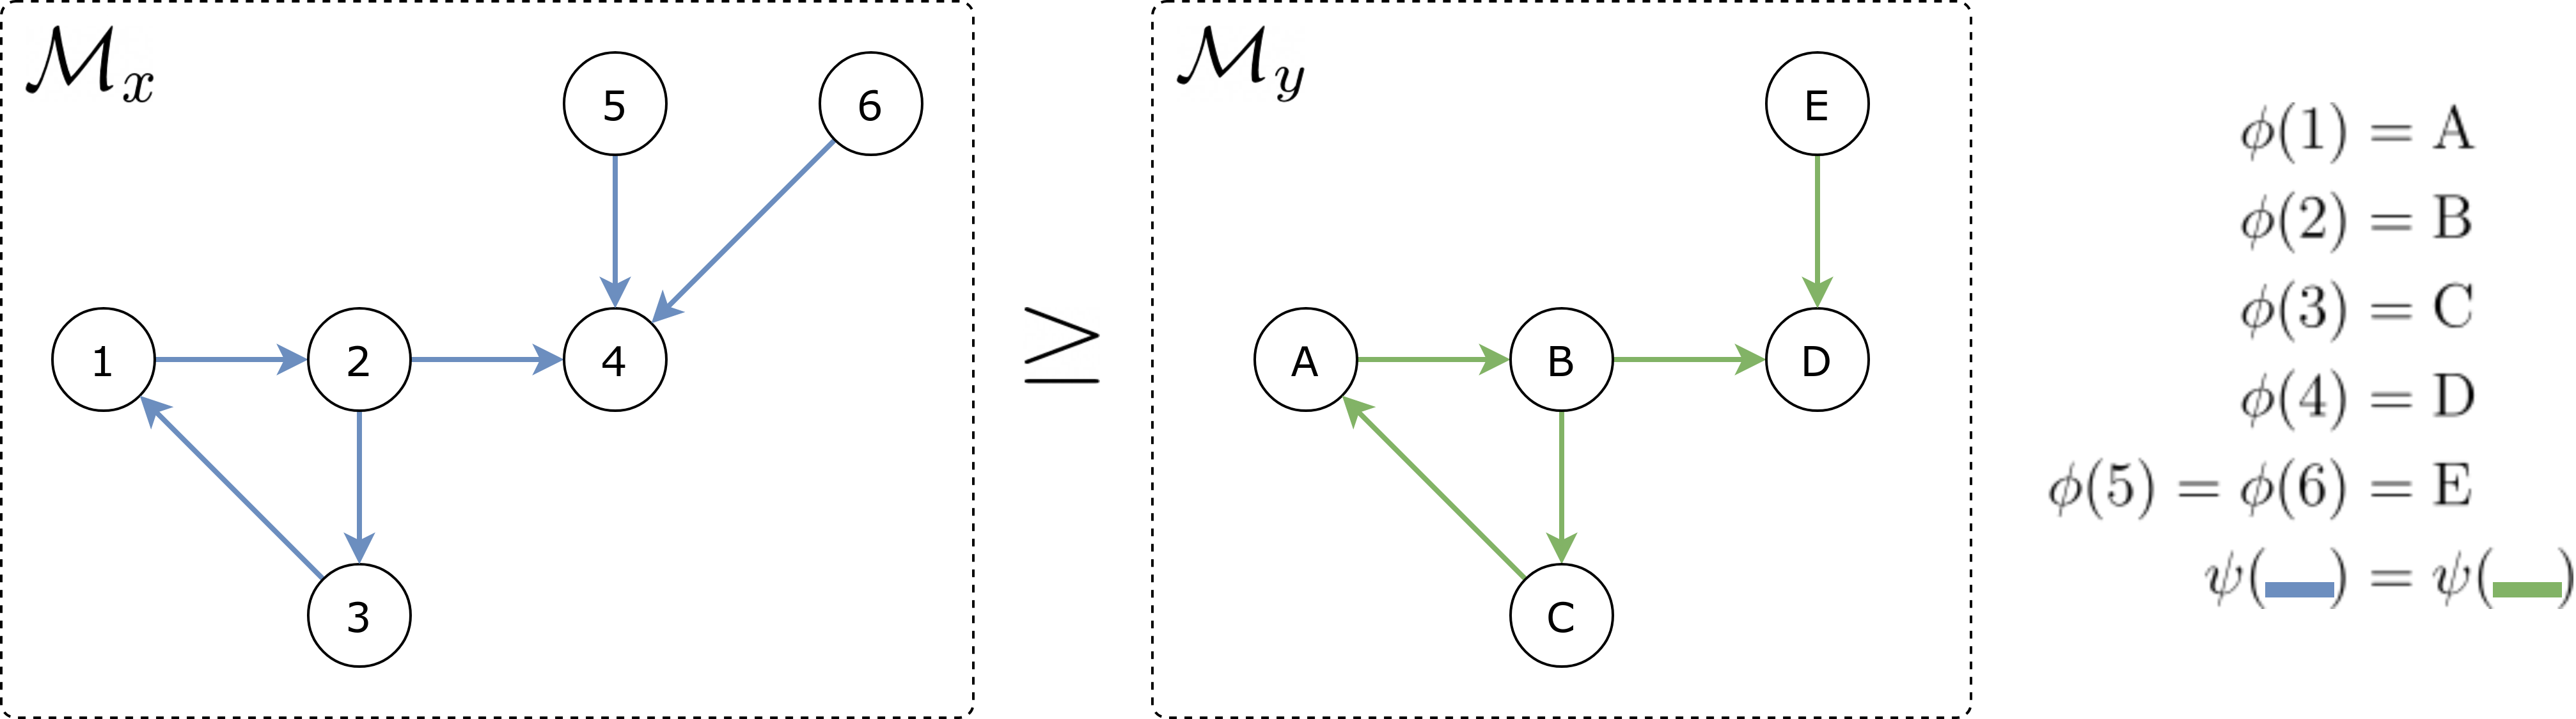
\includegraphics[width=0.9\linewidth]{\FigsDir/MDP_Reduction.png}
  \caption{An example of two MDPs for $x$ and $y$ domains where $\mathbb{M}_x \ge \mathbb{M}_y$. $\phi: \mathcal{S}_x \to \mathcal{S}_y$ and $\psi: \mathcal{A}_x \to \mathcal{A}_y$ are state and actions maps, respectively. States correspond to nodes and actions to colors. States 5, 6 in $\mathcal{S}_x$ are merged to state $e$ in $\mathcal{S}_y$ and blue actions in $\mathcal{A}_x$ are mapped to green actions in $\mathcal{A}_y$.}
  \label{ch:DAIL:fig:MDP_Reduction}
\end{figure}


\section{The Proposed \DAIL{} Agent\label{ch:DAIL:sec:Proposal}}
In this section,
the proposed \DAIL{} agent is introduced.
The agent relies on learning the domain-shared and domain-specific features in order to recover expert behaviors and adapt them to the learner agent domain.
The architecture of the proposed agent is illustrated in Figure \ref{ch:DAIL:fig:Architecture}.
The agent includes three deep feed-forward networks $F$, $G$, and $D$ that holds different responsibilities.

\begin{figure}[htbp!]
  \centering
  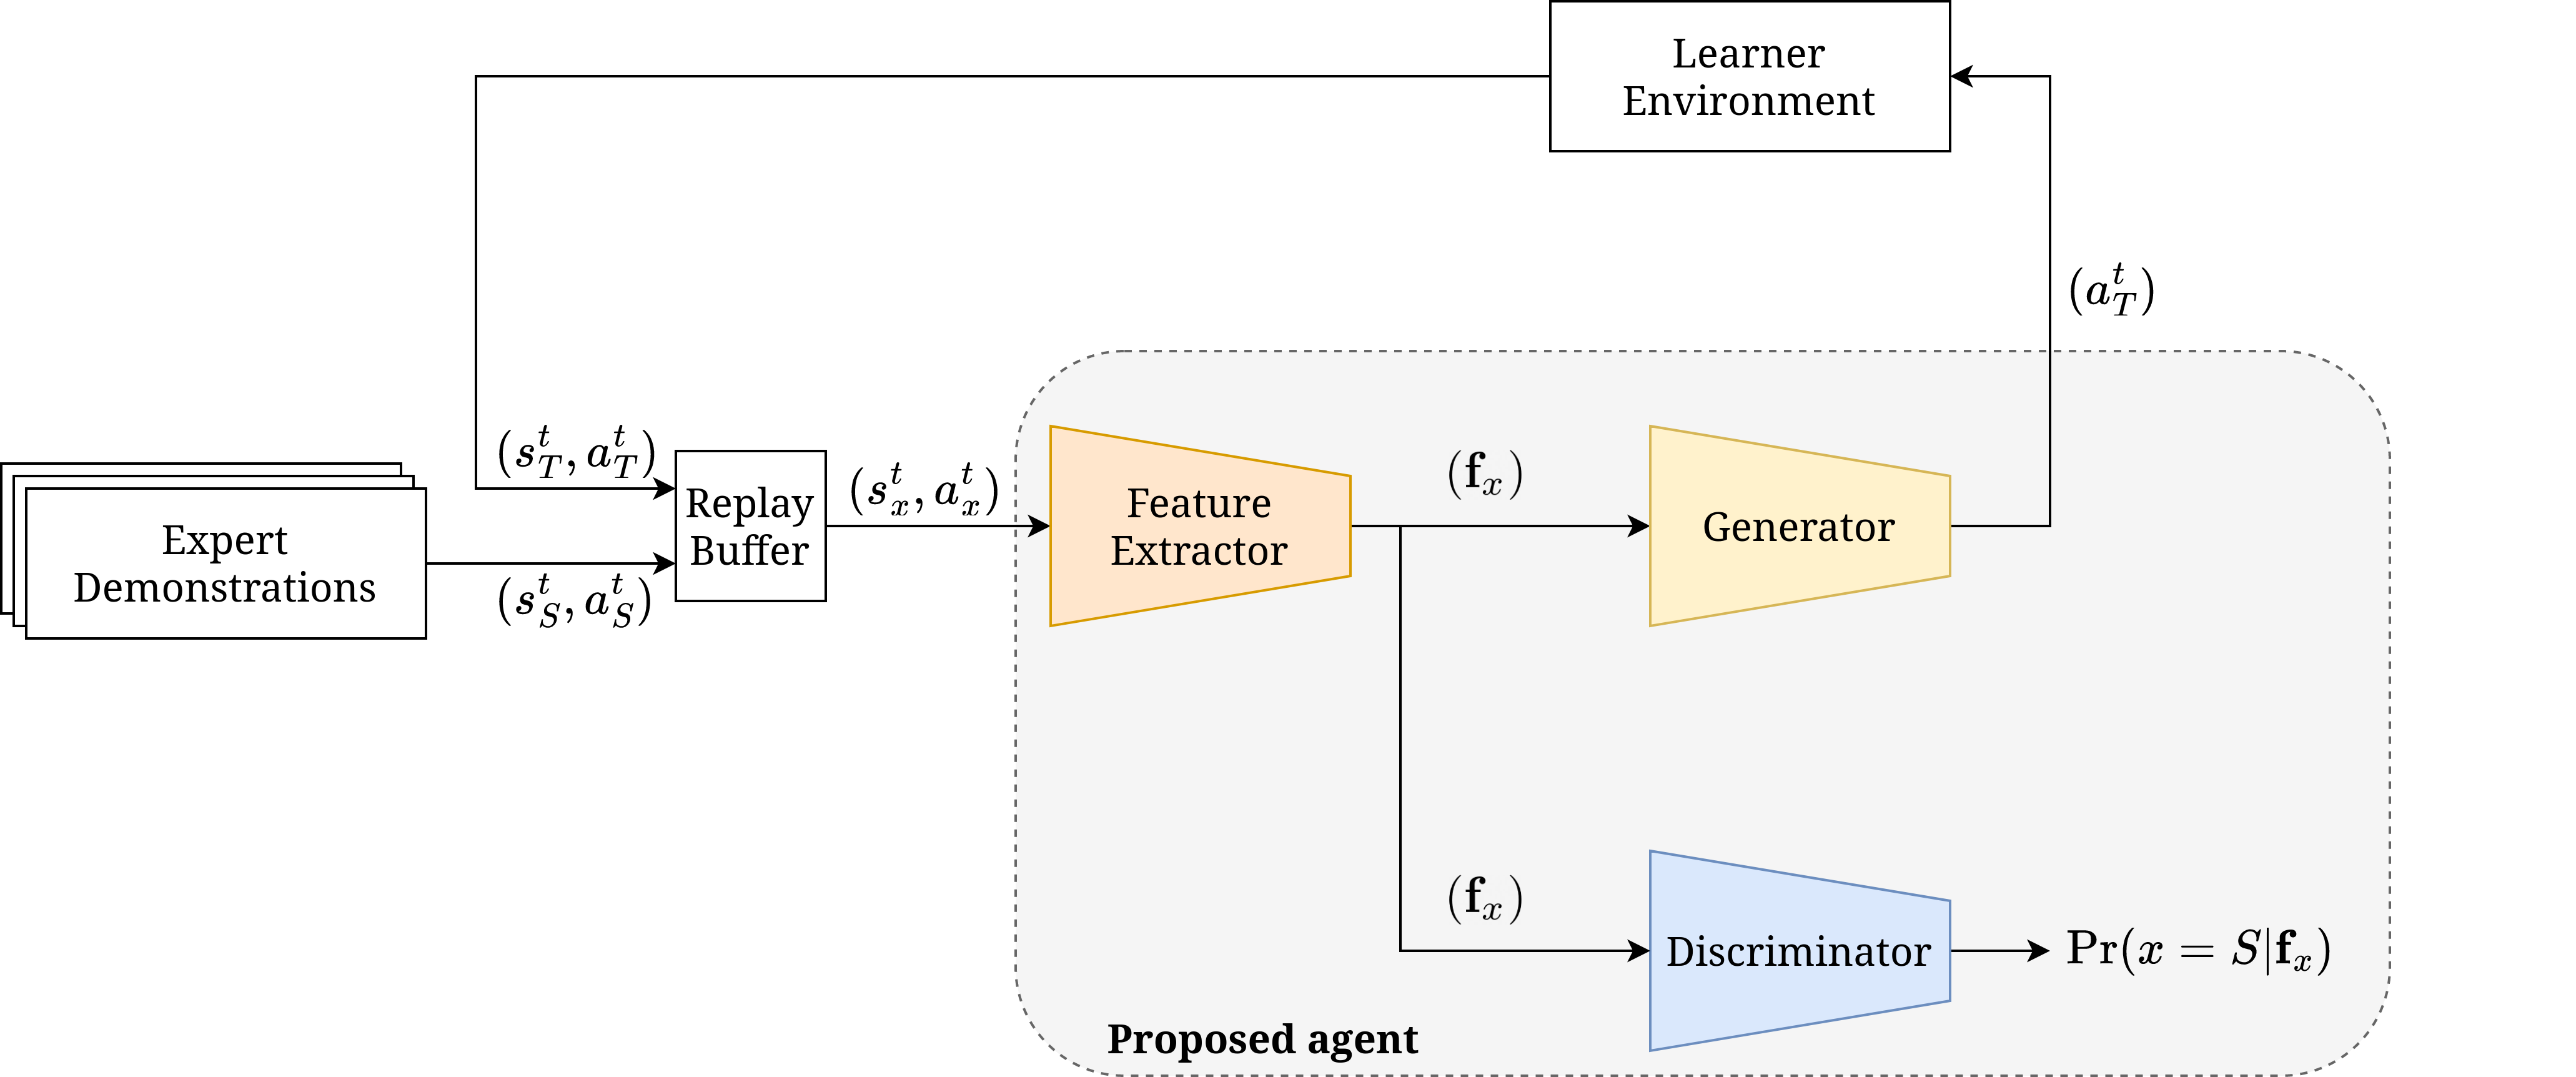
\includegraphics[width=\linewidth]{\FigsDir/new_Architecture.png}
  \caption{\added{The neural network architecture of the proposed \DAIL{} agent.}}
  \label{ch:DAIL:fig:Architecture}
\end{figure}

\subsection{Feature Extractor Network \texorpdfstring{$F$}{F}}
A state-action pair $(s^t_x, a^t_x)$ in domain $x$ is \added{sampled from a replay buffer \cite{zhang2017deeper} and} input to the feature extractor $F$ to produce a feature vector $\mathbf{f}_x=F(s^t_x, a^t_x)$.
$F$ is trained to capture the structural similarities or the shared features between $\mathcal{E}$ and $\mathcal{L}$ domains by minimizing the distance between two features $\mathbf{f}_\mathcal{E}$ and $\mathbf{f}_\mathcal{L}$.
Therefore, the loss function of $F$ is defined as:

\begin{align}
  \mathfrak{L}_F (F, G) & = \mathbb{E} \left[ \left\|
    F(s^t_\mathcal{E}, a^t_\mathcal{E}) - F(s^t_\mathcal{L}, a^t_\mathcal{L})
  \right\| \right]                                    \\
                        & = \mathbb{E} \left[ \left\|
    F(s^t_\mathcal{E}, a^t_\mathcal{E}) - F( s^t_\mathcal{L}, G( F( s^t_\mathcal{E}, a^t_\mathcal{E} ) ) )
    \right\| \right]
  % 1/T \sum^{}_{}{|| f() - f() ||^2_2}
\end{align}


\subsection{Discriminator Network \texorpdfstring{$D$}{D} and Generator Network \texorpdfstring{$G$}{G}}
The discriminator $D$ is designed to distinguish between expert feature vector $\mathbf{f}_\mathcal{E}$ and learner feature vector $\mathbf{f}_\mathcal{L}$.
Specifically,
$D$ receives a feature vector $\mathbf{f}_x$ outputs a probability $\mathrm{Pr}(x=\mathcal{E}|\mathbf{f}_x)$ to classify whether $\mathbf{f}_x$ is from $\mathcal{E}$ or $\mathcal{L}$.
Meanwhile,
the generator $G$ aims to generate an action $a^t_{L}$ so that $\mathbf{f}_\mathcal{L} = F(s^t_\mathcal{L}, a^t_\mathcal{L})$ looks as similar as possible to $\mathbf{f}_\mathcal{E}$.
In the proposed \DAIL{} agent,
the adversarial loss \cite{GAN_Original} is applied for both networks:

\begin{align}
  \mathfrak{L}_{GAN}(G, D) & =
  \mathbb{E}[
    \log{D(F(s^t_\mathcal{E}, a^t_\mathcal{E}))}
  ] + \mathbb{E}[
    \log{(1-D(F(s^t_\mathcal{L}, a^t_\mathcal{L})))}
  ]                                        \\
                           & = \mathbb{E}[
    \log{D(F(s^t_\mathcal{E}, a^t_\mathcal{E}))}
  ] + \mathbb{E}[
    \log{(1-D(F(s^t_\mathcal{L}, G(F(
      s^t_\mathcal{E}, a^t_\mathcal{E}
      )))))}
  ]
\end{align}

The optimal policy is achieved using a RL-based policy gradient,
which relies on reward signal $r=-\log{D(F(s^t_\mathcal{E}, a^t_\mathcal{E}))}$ provided by the learned discriminator.


\subsection{Full Objective}
During the learning phase,
in order to learn domain-shared features between $\mathcal{E}$ and $\mathcal{L}$ domains,
the feature extractor $F$ and the generator $G$ are optimized to minimize the feature extractor loss $\mathfrak{L}_F$.
At the same time,
given a feature vector $\mathbf{f}_x$ of domain $x$,
we want to judge whether $\mathbf{f}_x$ is from $\mathcal{E}$ or $\mathcal{L}$ by minimizing the domain classification loss $\mathfrak{L}_{GAN}$.
This encourages domain-specific features to be captured by $F$.
Overall, the full objective function is:

\begin{align}
   & \underset{F, G}{max} \underset{D}{min} \mathfrak{L}(F, G, D) \\
   & \quad\text{subject to \:}
  \mathfrak{L}(F, G, D) = {\mathfrak{L}_{GAN}(G, D)} - \lambda\mathfrak{L}_F
\end{align}

The goal is to find a saddle point, where:

\begin{align}
  (\hat{F}, \hat{G}) & = \underset{F, G}{argmax}{\mathfrak{L}(F, G, \hat{D})}    \\
  \hat{D}            & = \underset{D}{argmin}{\mathfrak{L}(\hat{F}, \hat{G}, D)} \\
\end{align}

At the saddle point,
the $\hat{D}$ minimizes the domain classification loss.
The feature extractor $\hat{F}$ and the generator $\hat{G}$ minimize the distance between both domains (i.e. the features are shared between domains),
while maximizing the domain classification loss (i.e. the features are specific to each domain).
The parameter $\lambda$ controls the trade-off between domain-shared features and domain-specific features should be learned by $F$.

The learning algorithm of the proposed agent is outlined in Algorithm \ref{ch:DAIL:alg:ProposedModel}.

\begin{algorithm}
  \caption{\DAIL{}}
  \label{ch:DAIL:alg:ProposedModel}

  \begin{algorithmic}[1]
    \Input
    \Desc{$\mathcal{D}_\mathcal{E}$}{A set of expert demonstrations}
    \EndInput

    \State Randomly initialize feature extractor network $F$, generator $G$ and discriminator $D$
    \For {i = 0, 1, 2, ...}
    \State Sample an expert demonstration $\tau^i_\mathcal{E} \sim \mathcal{D}_\mathcal{E}$
    \State Update the parameters of feature extractor network $F$ with the gradient
    \[\mathbf{E}[
        \nabla_F log(D( \mathbf{f}_\mathcal{E} ))
      ] + \mathbf{E}[
        \nabla_F log(1 - D( \mathbf{f}_\mathcal{L} ))
      ] - \lambda \mathbf{E}[
        \nabla_F \left\|
        \mathbf{f}_\mathcal{E} - \mathbf{f}_\mathcal{L}
        \right\|
      ]
    \]
    \State Update the discriminator parameters with the gradient
    \[\mathbf{E}[
        \nabla_D log(D( \mathbf{f}_\mathcal{E} ))
      ] + \mathbf{E}[
        \nabla_D log(1 - D( \mathbf{f}_\mathcal{L} ))
      ]\]
    \State Update policy $\pi_{L}$ with the reward signal $r=-logD(\mathbf{f}_\mathcal{E})$
    \EndFor

    \Output
    \Desc{$\pi_{L}$}{Learned policy for learner domain}
    \EndOutput
  \end{algorithmic}
\end{algorithm}




\section{Performance Evaluation\label{ch:DAIL:sec:Evaluation}}
In this section, the performance of the proposed \DAIL{} agent is evaluated by comparing with various baseline agents on a number of tasks ranging from low to complex high-dimensional.
The details of the experimental settings and evaluation results are presented in the following subsections.

\subsection{Experimental Settings}
\subsubsection{Environments}

In this experiment,
five simulated environments were considered:
Pendulum \cite{Task_OpenAIGym},
Acrobot \cite{Task_OpenAIGym,Task_Acrobot1,Task_Acrobot2},
CartPole \cite{Task_OpenAIGym,Task_CartPole},
Door \cite{Task_Adroit},
and Hammer \cite{Task_Adroit}.
The detailed descriptions and visualizations of these environment are shown in Table \ref{ch:DAIL:tab:Tasks} and Figure \ref{ch:DAIL:fig:EnvVisualization},
respectively.
From such environments,
five domain adaptive tasks were decided,
each of which included two different environments - an expert domain and a learner domain.
These tasks can be divided into 2 categories as follows:

\begin{itemize}
  \item \textbf{Low-dimensional tasks}:
        \begin{itemize}
          \item Pendulum-Acrobot: Expert domain is Pendulum and learner domain is Acrobot.
          \item Pendulum-CartPole: Expert domain is Pendulum and learner domain is CartPole.
          \item Acrobot-CartPole: Expert domain is Acrobot and learner domain is CartPole.
        \end{itemize}
        To provide expert demonstrations,
        for each task,
        the Trust Region Policy Optimization method \cite{RL_TRPO} is first trained on the expert domain using the shaped reward signal.
        Then,
        20 expert demonstrations are collected by executing the learned policies in the expert domain simulator.
        Each demonstration includes a sequence of state-action pairs.
        It should be noted that only successful demonstrations where the learned policies can accomplish the task are collected.

  \item \textbf{High-dimensional tasks}:
        \begin{itemize}
          \item Door-Door: The expert and learner domains have different friction parameter. The friction parameter in expert domain is $[1, 1, 1]$, while in learner domain is $[4.0, 4.0, 4.0]$.
          \item Hammer-Hammer: The expert and learner domains have different mass of the hammer. The mass of the hammer in expert domain is 0.253442, while in learner domain is 1.0.
        \end{itemize}
        Twenty expert demonstrations are used for each task.
        The demonstrations are collected from humans using the Mujoco HAPTIX system \cite{Mujoco_HAPTIX} and publicly available \cite{Task_Adroit}.
\end{itemize}

\begin{landscape}
  \begin{table}[htbp!]
    \centering
    \caption{Description of five simulated environments used in the experiment.}
    \label{ch:DAIL:tab:Tasks}
    \begin{tabular}{cccp{8cm}}
  \toprule
  \textbf{Task}                                             & \textbf{State space} & \textbf{Action space} & \textbf{Description}                                                       \\
  \midrule
  Pendulum \cite{Task_OpenAIGym}                            & 3 (continuous)       & 1 (continous)         & Swinging up a pendulum.                                                    \\
  Acrobot \cite{Task_OpenAIGym,Task_Acrobot1,Task_Acrobot2} & 6 (continuous)       & 3 (discrete)          & Swinging the end of the lower link up to a given height                    \\
  CartPole \cite{Task_OpenAIGym,Task_CartPole}              & 4 (continuous)       & 2 (discrete)          & Preventing the pendulum from falling over by applying a force to the cart. \\

  Door \cite{Task_Adroit}                                   & 39 (continuous)      & 28 (continuous)       & A 24-DoF hand attempts to undo the latch and swing the door open.          \\
  Hammer \cite{Task_Adroit}                                 & 46 (continuous)      & 26 (continous)        & A 24-DoF hand attempts to use a hammer to drive the nail into the board.   \\
  \bottomrule
\end{tabular}

  \end{table}

  \begin{table}[htbp!]
    \centering
    \caption{\DAIL{} hyperparameters used in the experiment. Each number corresponds to the number of nodes in a network layer.}
    \label{ch:DAIL:tab:ModelHyperparameteres}
    
\begin{tabular}{lccc}
  \toprule
  \textbf{}              & \textbf{Feature Extractor $F$}    & \textbf{Generator $G$}                            & \textbf{Discriminator $D$}      \\
  \midrule
  Low-dimensional Tasks  & $(s^t_x, a^t_x)$ - 32 - 32 - 16   & $(\mathbf{f}_x)$ - 32 - 32 - $(a^t_\mathcal{L})$  & $(\mathbf{f}_x)$ - 32 - 32 - 1  \\
  High-dimensional Tasks & $(s^t_x, a^t_x)$ - 128 - 128 - 64 & $(\mathbf{f}_x)$ - 128 - 64 - $(a^t_\mathcal{L})$ & $(\mathbf{f}_x)$ - 128 - 64 - 1 \\
  \bottomrule
\end{tabular}

  \end{table}
\end{landscape}

\begin{figure}[htbp!]
  \centering
  \begin{subfigure}[b]{0.25\textwidth}
    \centering
    \frame{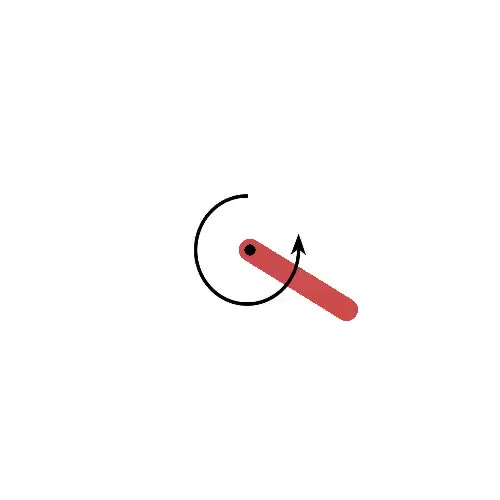
\includegraphics[width=\linewidth]{\FigsDir/Pendulum.jpg}}
    \caption{Pendulum}
  \end{subfigure}
  \hfill
  \begin{subfigure}[b]{0.25\textwidth}
    \centering
    \frame{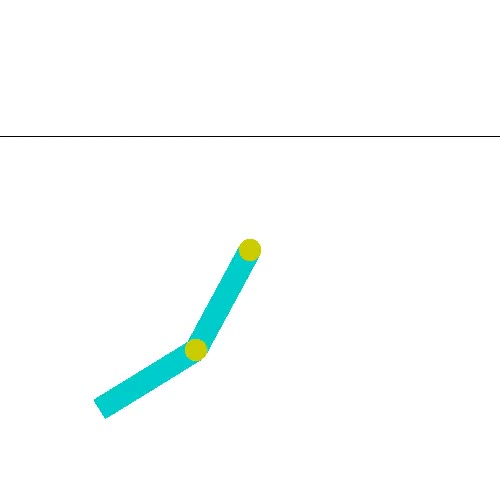
\includegraphics[width=\linewidth]{\FigsDir/Acrobot.jpg}}
    \caption{Acrobot}
  \end{subfigure}
  \hfill
  \begin{subfigure}[b]{0.25\textwidth}
    \centering
    \frame{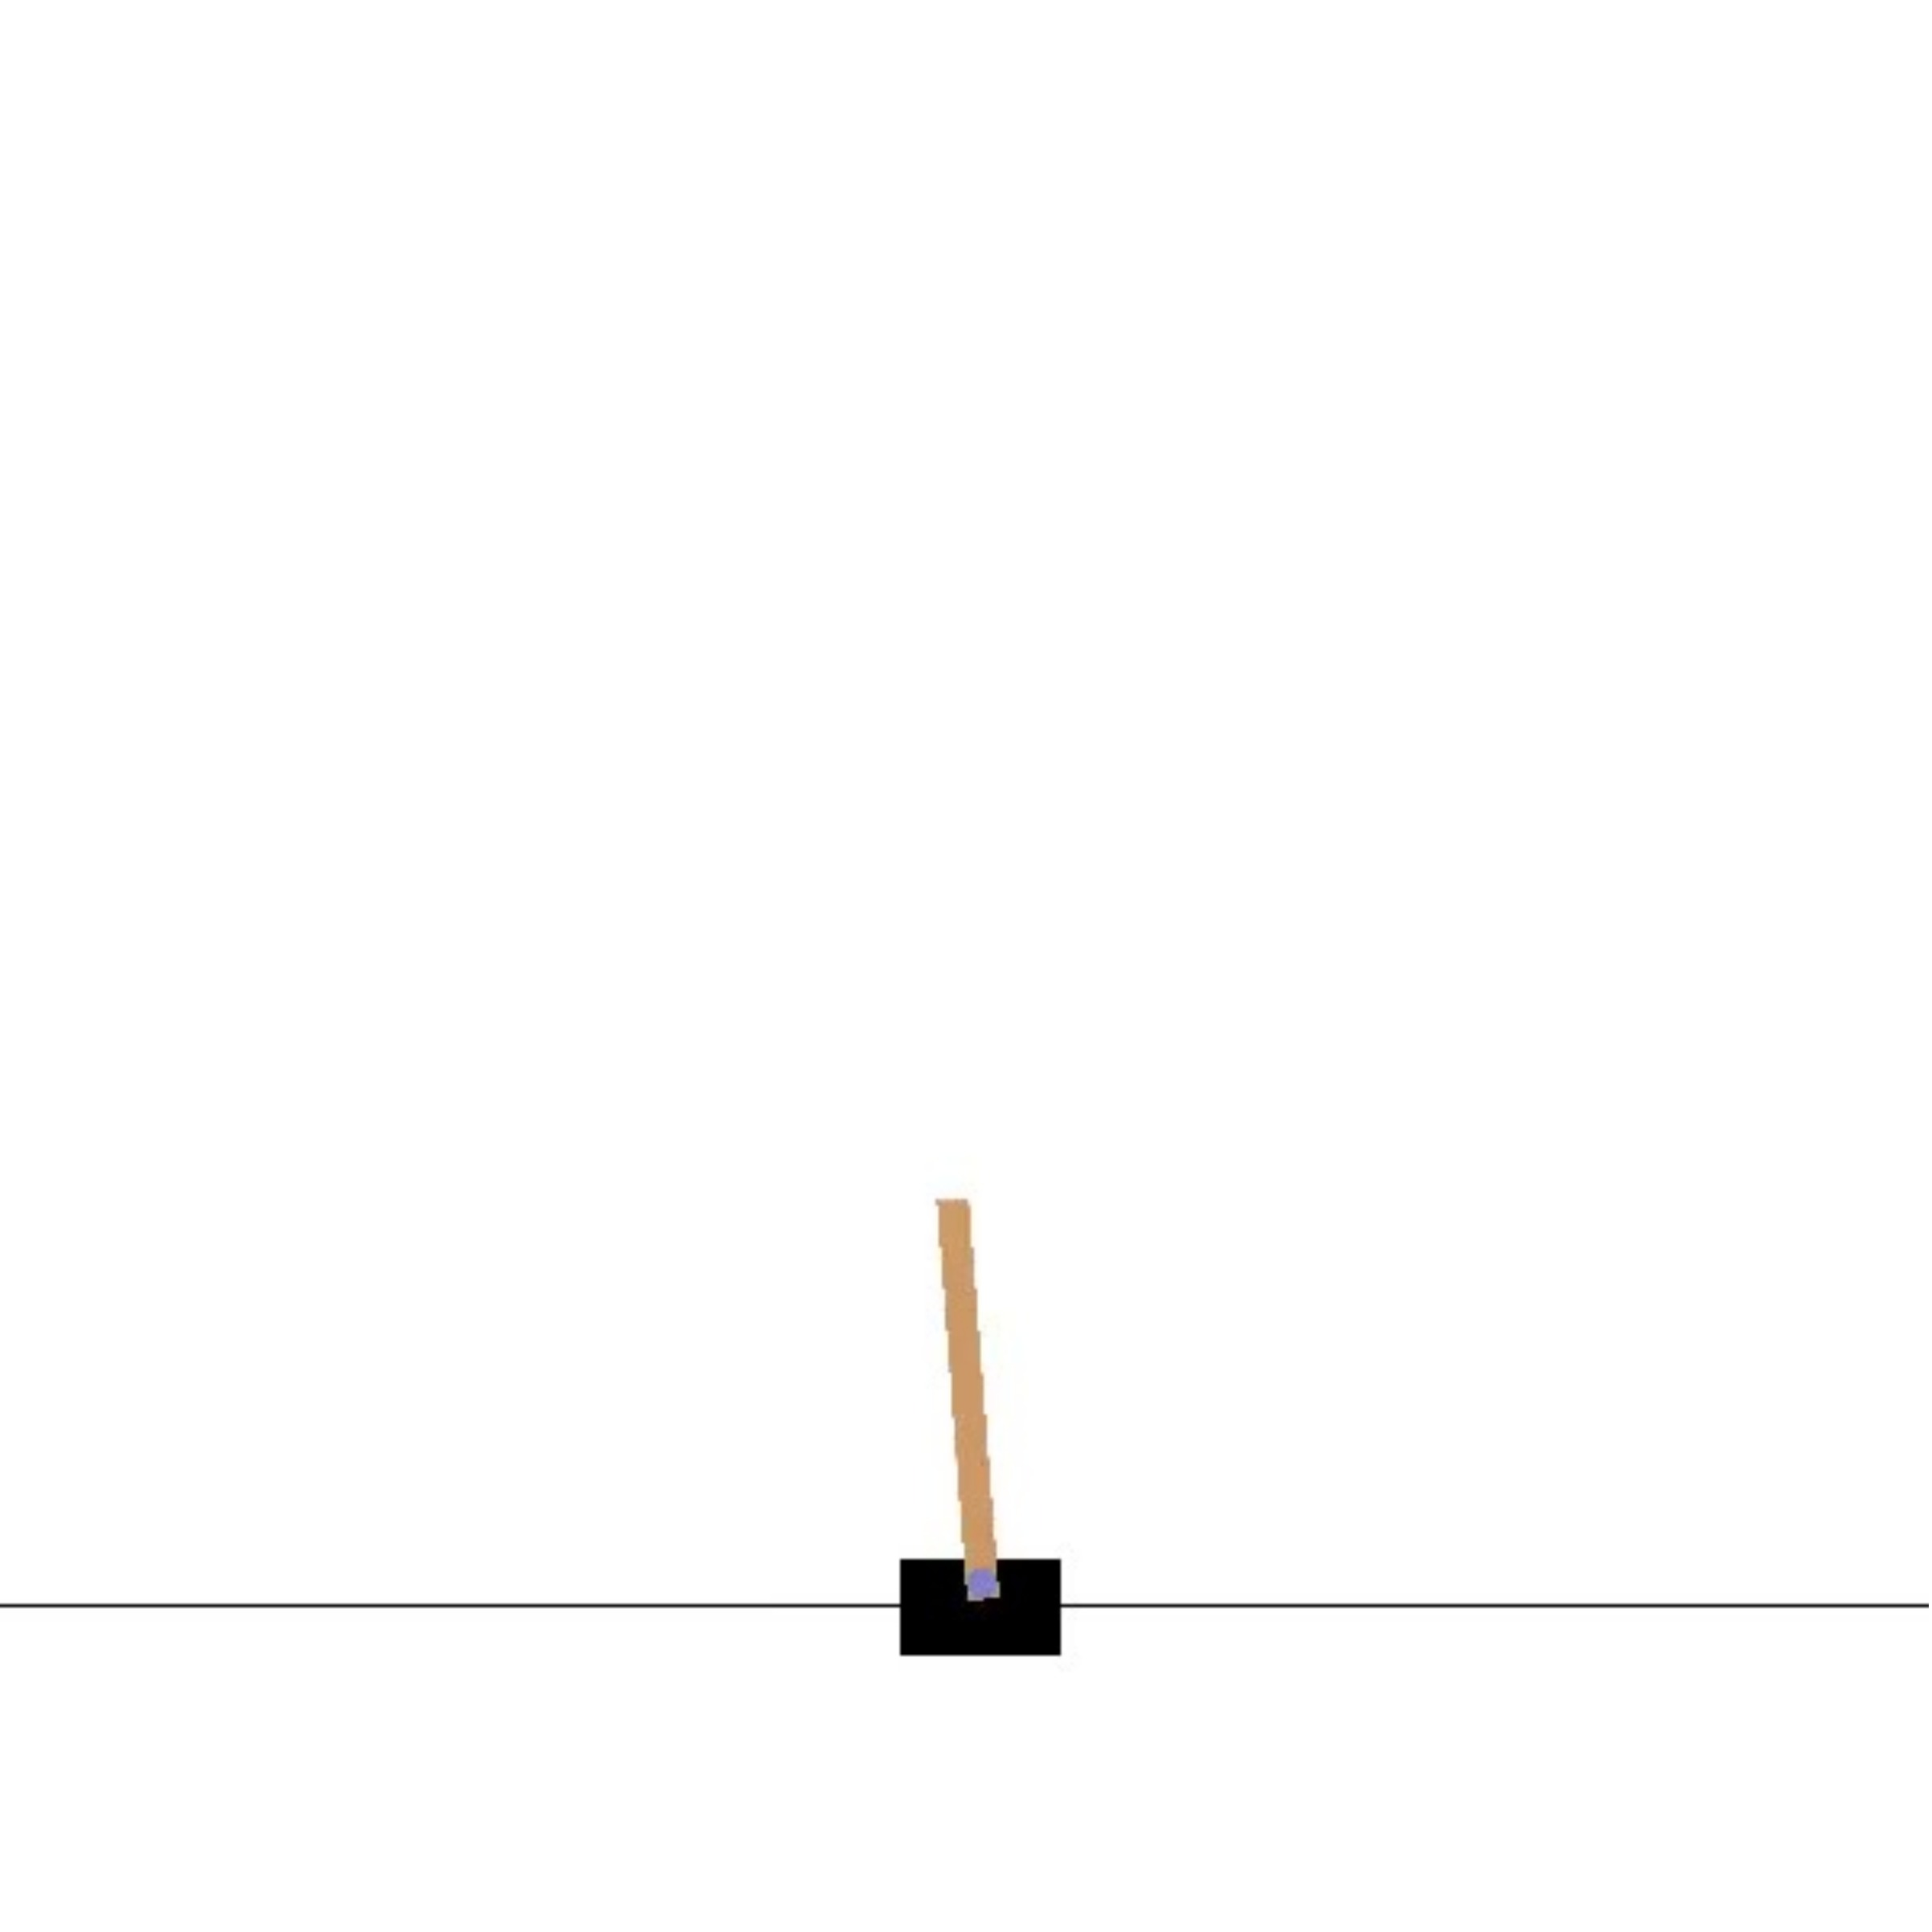
\includegraphics[width=\linewidth]{\FigsDir/CartPole.jpg}}
    \caption{CartPole}
  \end{subfigure}
  \par\bigskip
  \begin{subfigure}[b]{0.25\textwidth}
    \centering
    \frame{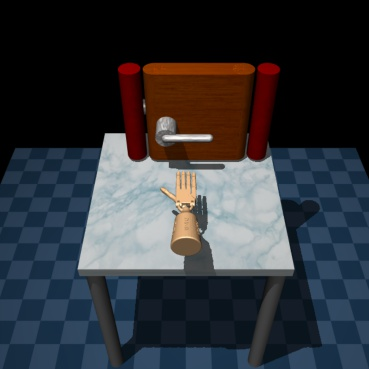
\includegraphics[width=\linewidth]{\FigsDir/Door.jpg}}
    \caption{Door}
  \end{subfigure}
  \hspace{4em}
  \begin{subfigure}[b]{0.25\textwidth}
    \centering
    \frame{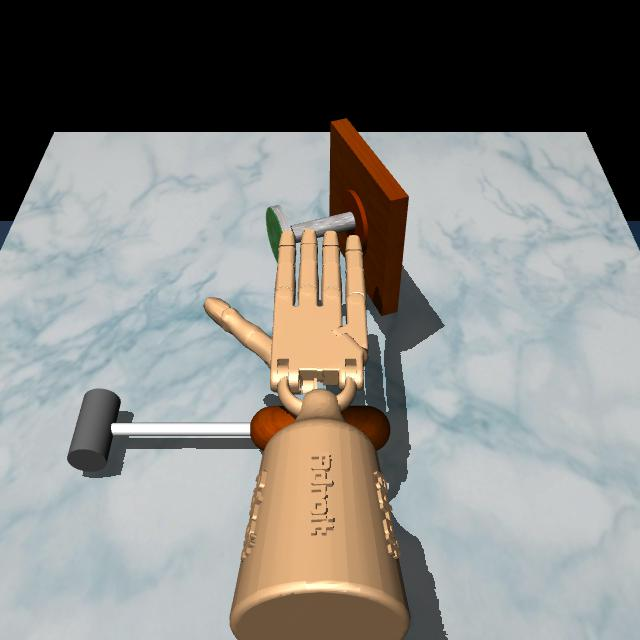
\includegraphics[width=\linewidth]{\FigsDir/Hammer.jpg}}
    \caption{Hammer}
  \end{subfigure}
  \caption{Visual rendering of five simulated environments used in the experiment.}
  \label{ch:DAIL:fig:EnvVisualization}
\end{figure}



%==================================================
\subsubsection{Baselines}

The performance of the proposed \DAIL{} agent was evaluated in comparison with the following baseline methods:

\begin{itemize}
  \item
        Trust Region Policy Optimization (TRPO) \cite{RL_TRPO} is a Reinforcement learning-based agent.
        The agent was trained directly on the learner domain and had access to the shaped reward function.
        This baseline set an upper bound for the performance of domain adaptation algorithms.

  \item
        GAMA-PA \cite{DAIL_Model_DAIL}:
        The agent introduced a two-step approach for domain adaptation in imitation learning.
        It first learns the state-action maps between expert and learner domains, and then utilizes it to learn an optimal policy.
        The agent parameters are employed as reported in \cite{DAIL_Model_DAIL} in order to ensure a fair comparison.
\end{itemize}

%==================================================
\subsubsection{Network Structure and Hyperparameters}

Deep feed-forward networks with 2 hidden layers are used for three $F$, $G$, $D$ networks of the proposed agent.
\added{Grid search was utilized in order to find an optimal set of network hyperparameters.
  Since high-dimensional tasks are more challenging compared to low-dimensional tasks,
  DAIL-GAN requires a higher number of nodes in each network layer in order to provide a high and consistent performance.}
The network hyperparameters are shown in Table \ref{ch:DAIL:tab:ModelHyperparameteres}.
In this experiment, the learning rate was 0.0003.
Adam was used as an optimizer.


\subsection{Results}
In this subsection, the evaluation results of the proposed \DAIL{} agent on low- and high-dimensional tasks are presented to highlight its superior capability in tackling domain adaptation problem in imitation learning.

\subsubsection{Low-dimensional Tasks}
Table \ref{ch:DAIL:tab:Reward_Simple} reports the quantitative evaluations of the proposed \DAIL{} agent on low-dimensional tasks, in terms of average cumulative rewards.
The numerical results clearly indicate that, for all evaluated tasks, TRPO \cite{RL_TRPO} provided the best performance as its average cumulative rewards were at the highest.
This was actually predictable because TRPO \cite{RL_TRPO} had direct access to states and shaped rewards of the learner domain.
On the other hand, inputs of GAMA-PA \cite{DAIL_Model_DAIL} and \DAIL{} were limited to expert demonstrations only.
As a result, their performances deteriorated compared to TRPO \cite{RL_TRPO}.
However, Table \ref{ch:DAIL:tab:Reward_Simple} also determines that the proposed \DAIL{} outperformed GAMA-PA \cite{DAIL_Model_DAIL} across all three tasks.
Additionally, for the Pendulum-Acrobot task, the proposed agent almost achieved as high performance as TRPO \cite{RL_TRPO}.
In order to understand the observed results more deeply, Figures \ref{ch:DAIL:fig:PendulumAcrobot}, \ref{ch:DAIL:fig:PendulumCartPole} and \ref{ch:DAIL:fig:AcrobotCartPole} visualize the behaviors of learned policies provided by the evaluated agents when performing the Pendulum-Acrobot, Pendulum-CartPole and Acrobot-CartPole tasks, respectively.

\begin{table}[htbp!]
  \centering
  \caption{\added{The performance of the proposed \DAIL{} agent on low-dimensional tasks. These scores represent the cumulative rewards obtained from executing a learned policy in the simulator, averaged over 100 episodes.}}
  \label{ch:DAIL:tab:Reward_Simple}
  % TRPO
% Pendulum:
%       Mean:  -135.73463514842086    Std:  83.24276932922322
% CartPole:
%       Mean:  497.13       Std:  28.55613944496
% Acrobot:
%       Mean:  -63.18       Std:  7.047524388038681

% GAMA
% Acrobot:
%       Mean: -386.31   Std: 49.20
% Pendulum-CartPole:
%       Mean:  144.03   Std:  89.08574016081361
% Acrobot-CartPole:
%       Mean: 1
% Our
% Acrobot:
%       Mean:  -83.31   Std:  32.61248073974134
% Pendulum-CartPole:
%       Mean:  289.74   Std:  171.20727905086278
% Acrobot-CartPole:
%       Mean:  153.86 Std:  81.79371294405652
%

\begin{tabular}{cccc}
  \toprule
  \textbf{Task}     & \textbf{\DAIL{}}    & \textbf{GAMA-PA\cite{DAIL_Model_DAIL}} & \textbf{TRPO} \cite{RL_TRPO} \\
  \midrule
  Pendulum-Acrobot  & -83.31 $\pm$  32.61 & -386.31 $\pm$ 49.20                    & -63.18 $\pm$  7.05           \\
  Pendulum-CartPole & 289.74 $\pm$ 171.21 & 144.03 $\pm$ 89.09                     & 497.13 $\pm$ 28.56           \\
  Acrobot-CartPole  & 153.86 $\pm$  81.79 & 93.05 $\pm$ 88.97                      & 497.13 $\pm$ 28.56           \\
  \bottomrule
\end{tabular}

\end{table}

\begin{landscape}
  \begin{figure}[htbp!]
    \centering
    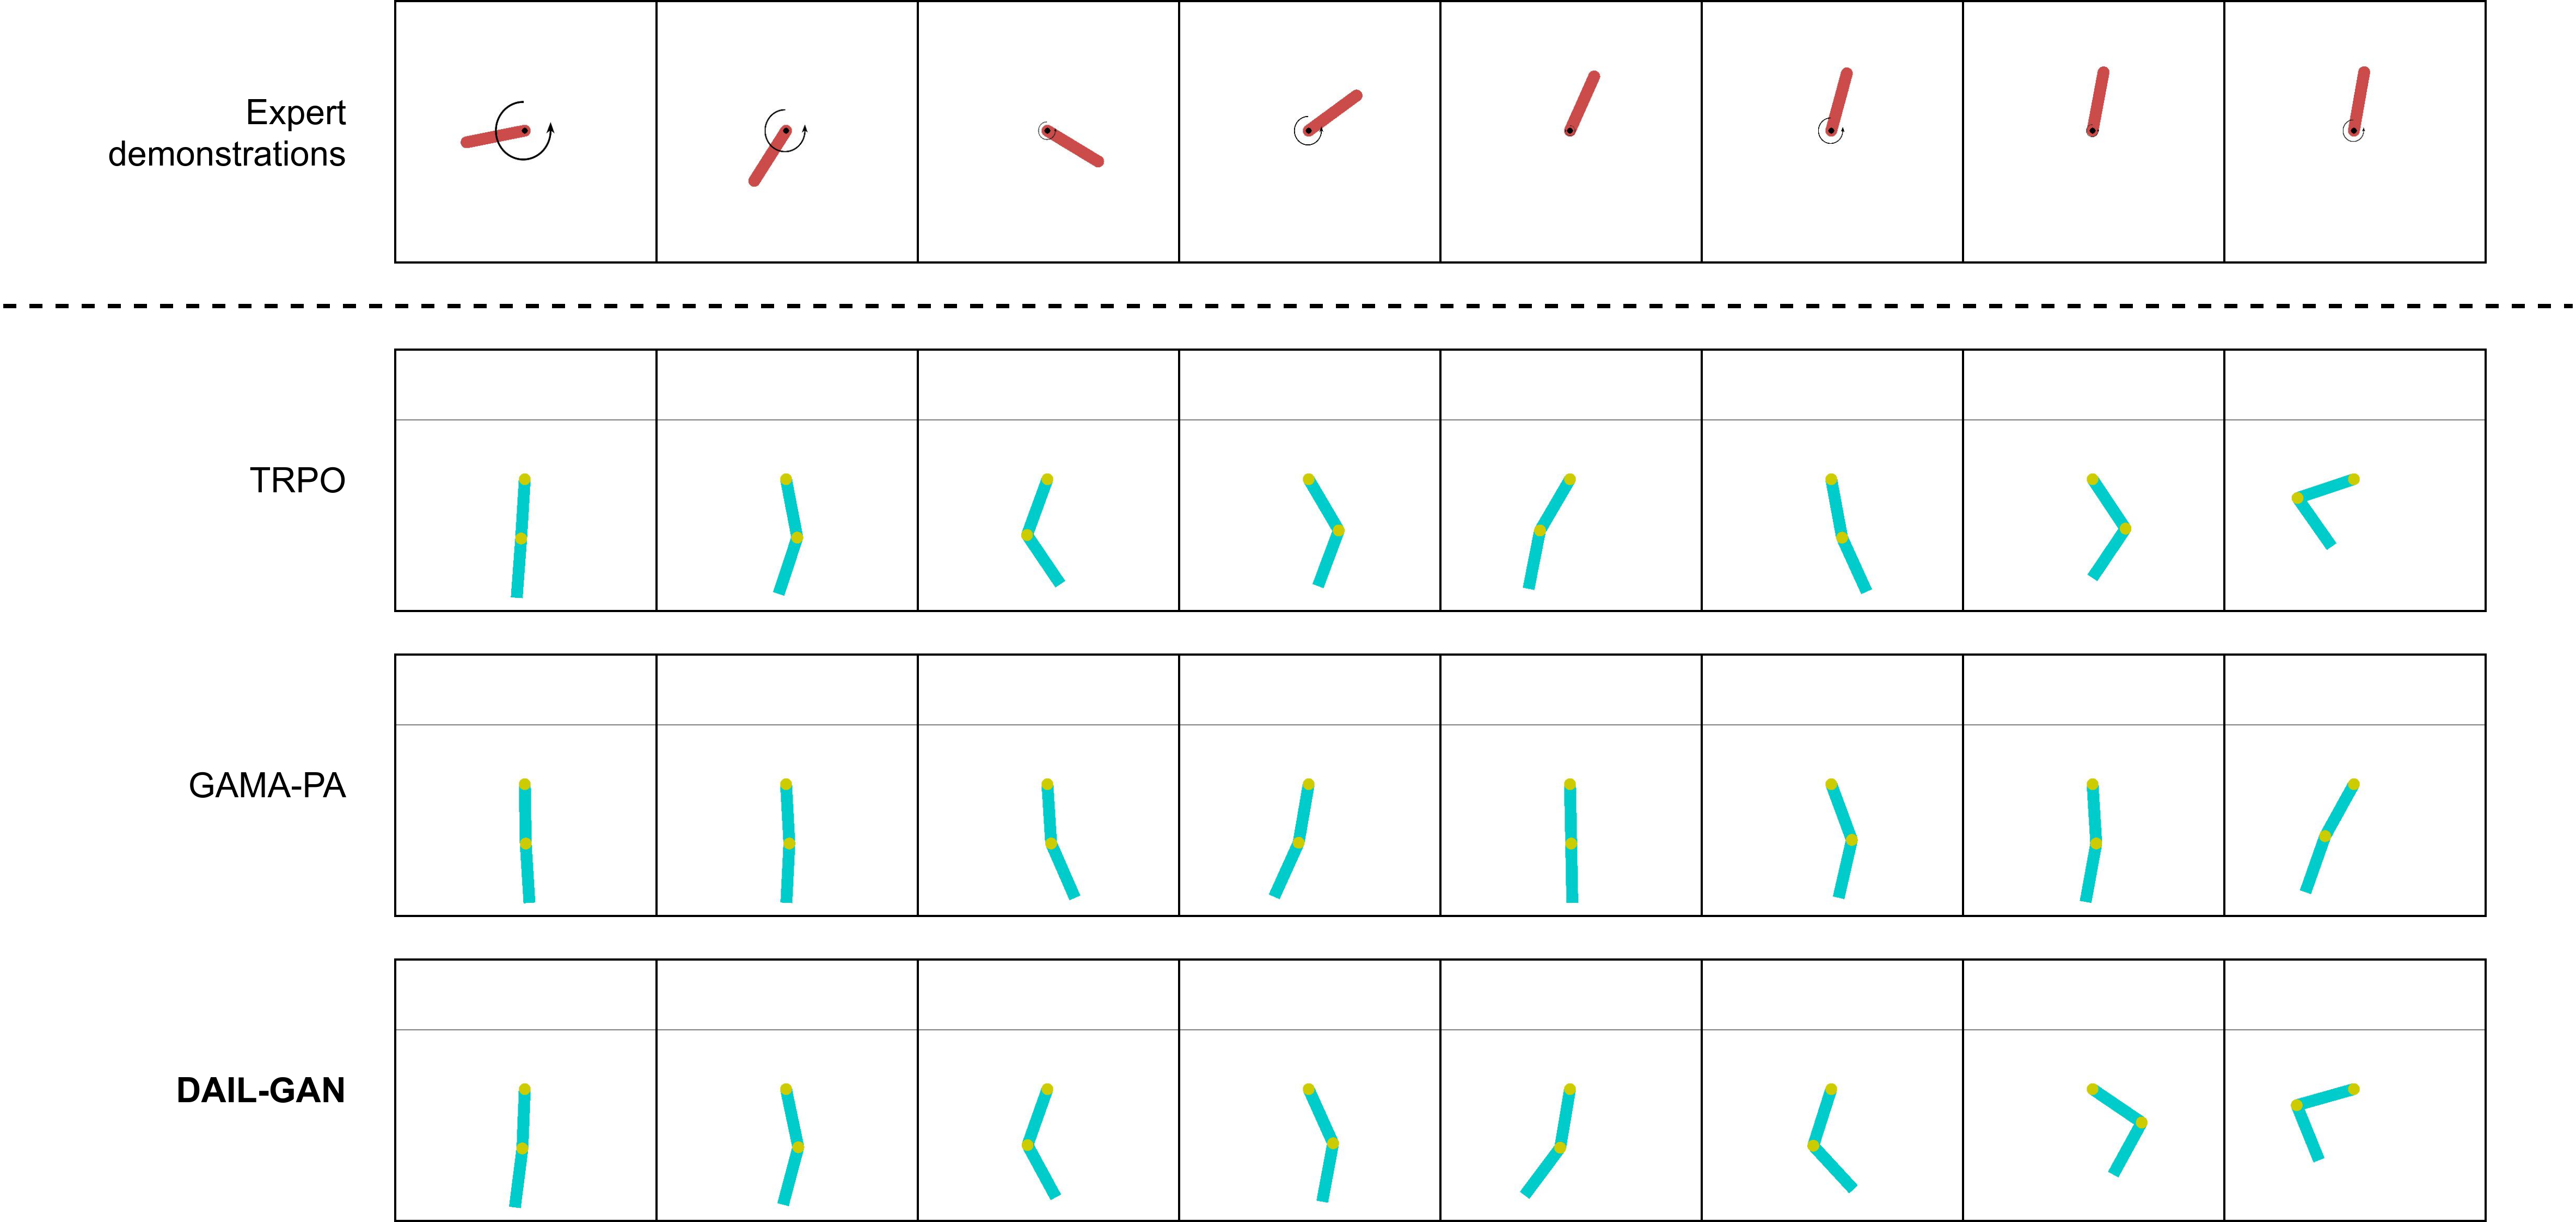
\includegraphics[width=0.7\pdfpageheight]{\FigsDir/Pendulum-Acrobot.png}
    \caption{Pendulum-Acrobot.}
    \label{ch:DAIL:fig:PendulumAcrobot}
  \end{figure}
\end{landscape}


\begin{landscape}
  \begin{figure}[htbp!]
    \centering
    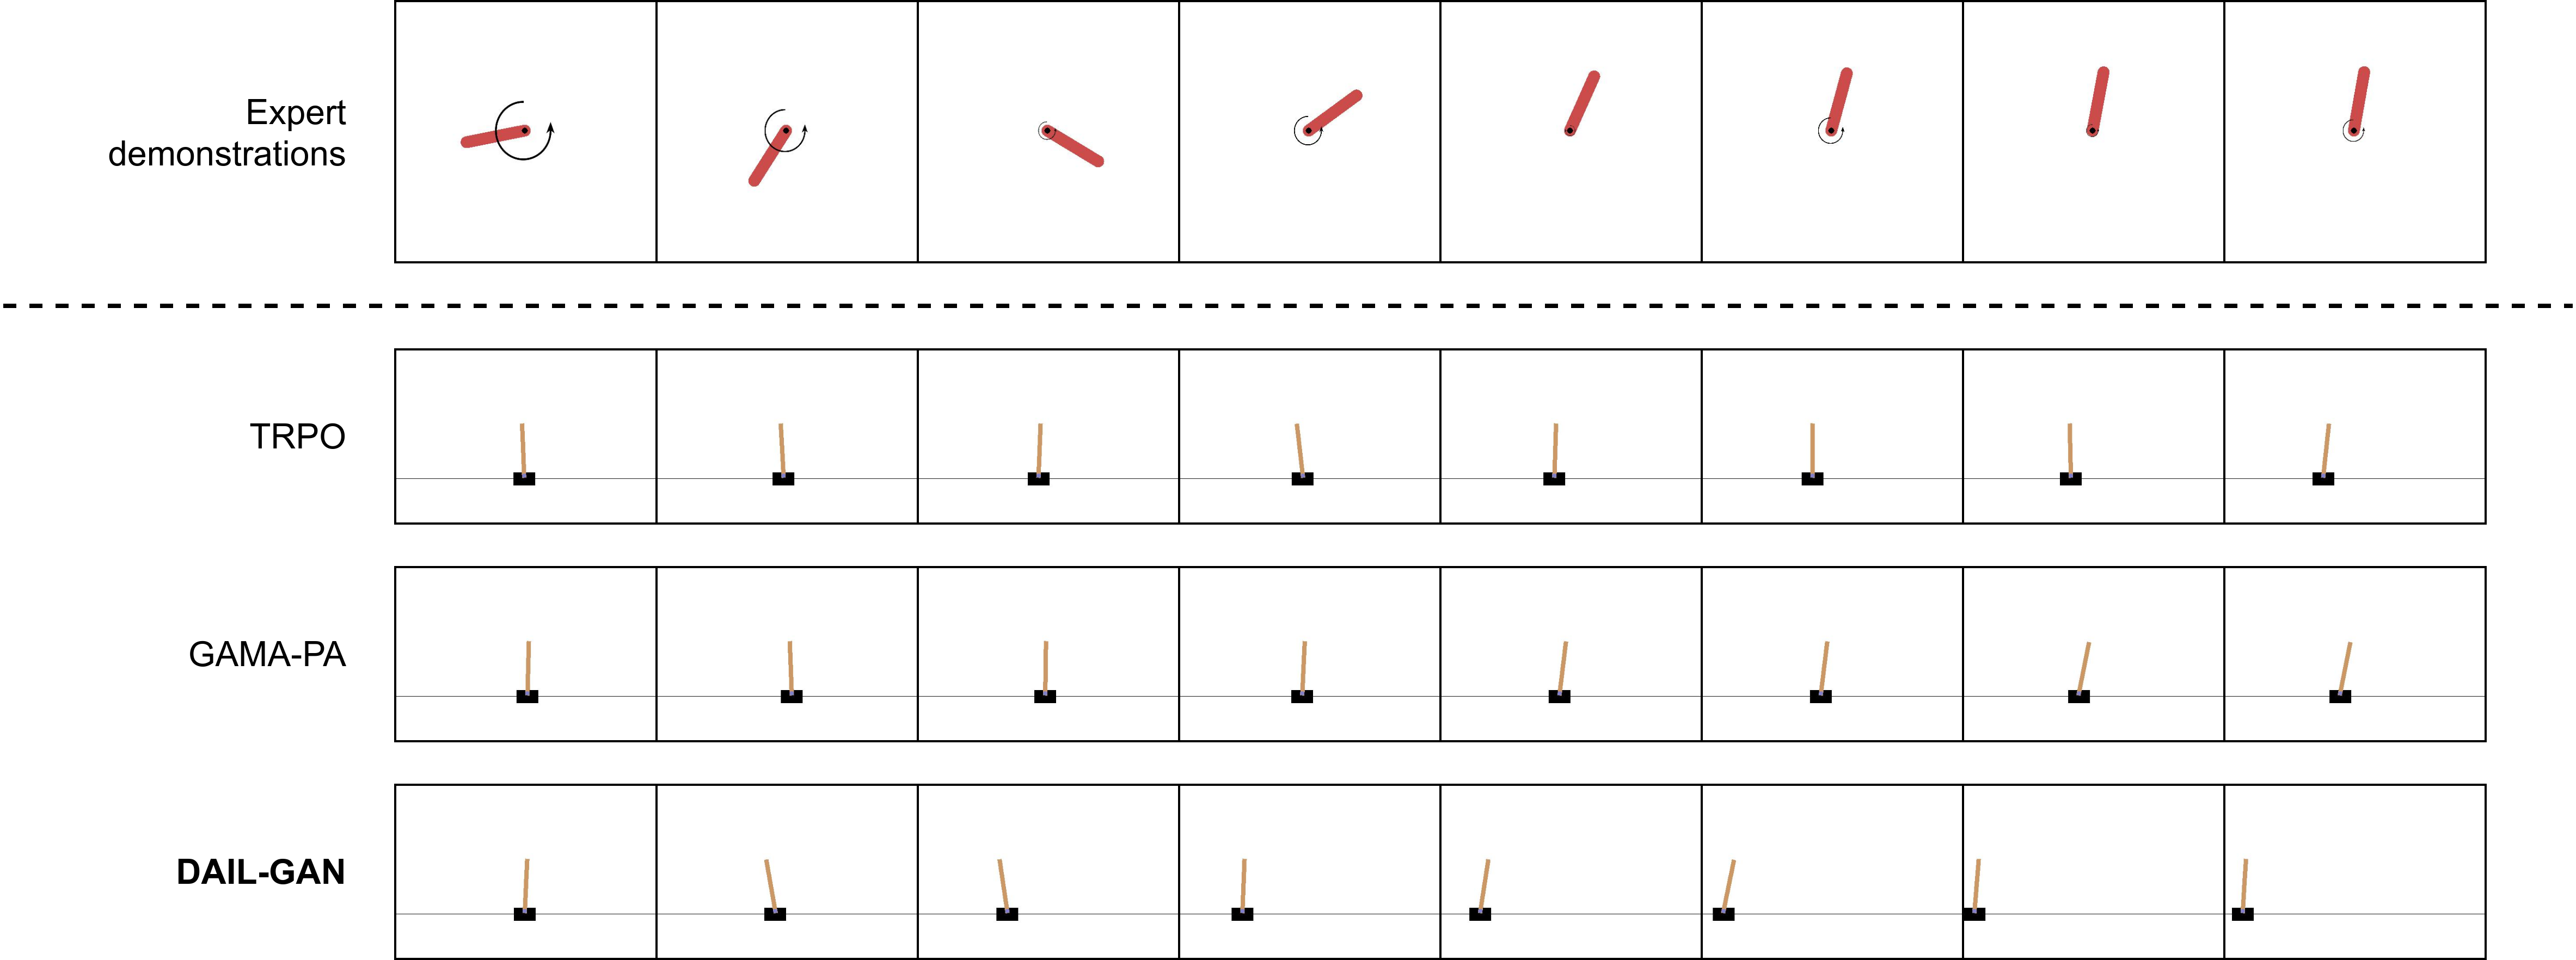
\includegraphics[width=0.7\pdfpageheight]{\FigsDir/Pendulum-CartPole.png}
    \caption{Pendulum-CartPole.}
    \label{ch:DAIL:fig:PendulumCartPole}
  \end{figure}
\end{landscape}

\begin{landscape}
  \begin{figure}[htbp!]
    \centering
    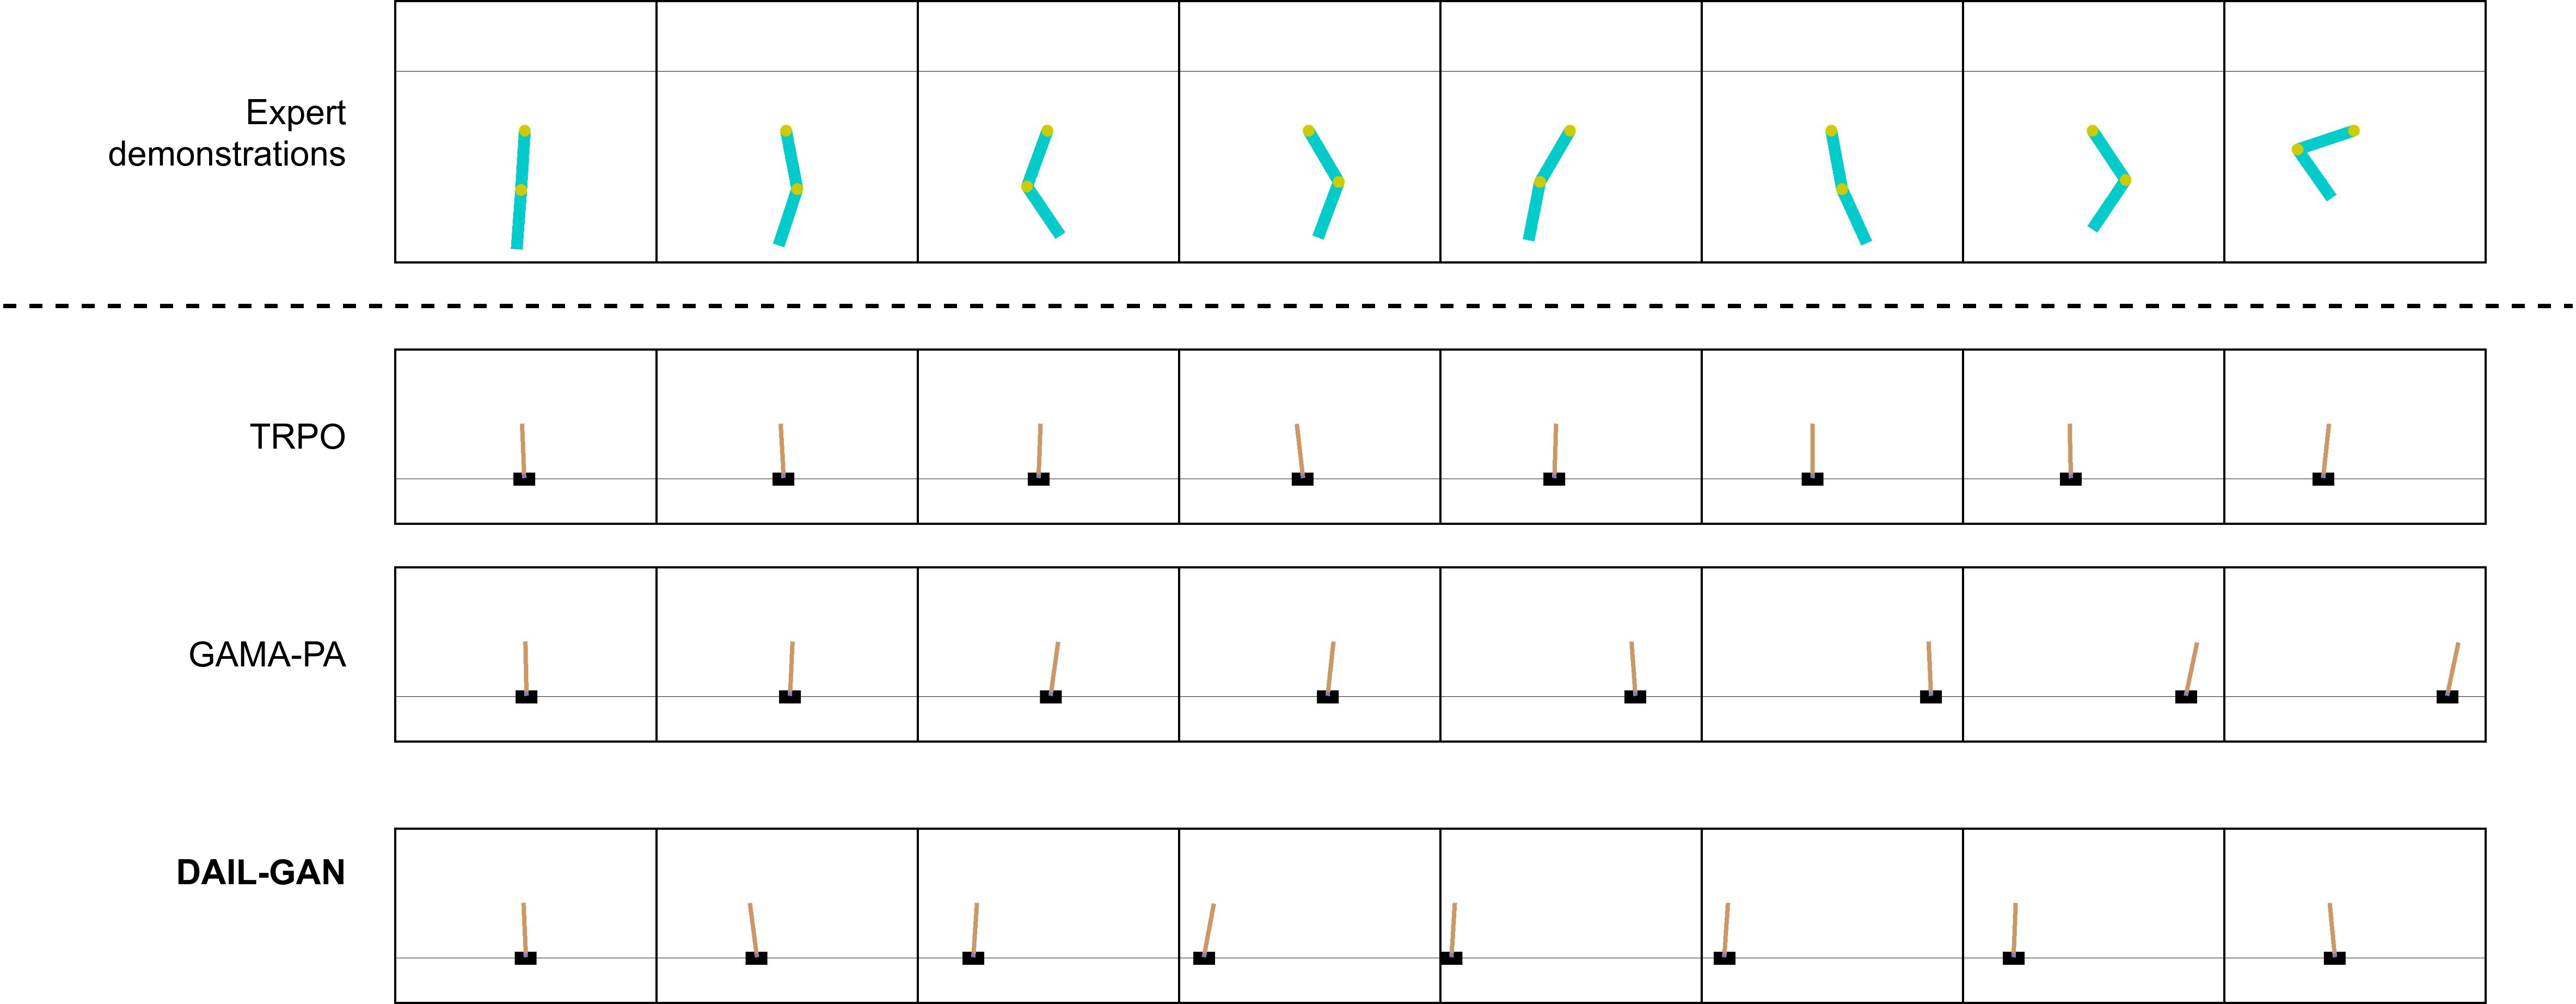
\includegraphics[width=0.7\pdfpageheight]{\FigsDir/Acrobot-CartPole.png}
    \caption{Acrobot-CartPole.}
    \label{ch:DAIL:fig:AcrobotCartPole}
  \end{figure}
\end{landscape}

In the expert demonstration of the Pendulum-Acrobot task in Figure \ref{ch:DAIL:fig:PendulumAcrobot} and the Pendulum-CartPole task in Figure \ref{ch:DAIL:fig:PendulumCartPole}, expert behaviors were to apply a strong force, expressed by a rotation velocity, at first to make the pendulum swing upright.
After that, a few light forces were applied to maintain it vertically.
Observing from Figure \ref{ch:DAIL:fig:PendulumAcrobot}, the policies trained with GAMA-PA \cite{DAIL_Model_DAIL} failed to apply strong enough forces to swing the lower link as high as the proposed DAIL.
Also, Figure \ref{ch:DAIL:fig:PendulumCartPole} expresses that the GAMA-PA \cite{DAIL_Model_DAIL} could not move the cart at an appropriate velocity to keep the pole stay vertical.
It was because the expert demonstration also did not show much movement after successfully swinging the pendulum upright as it only applied light forces.
Meanwhile, the policies learned by the \DAIL{} agent could accomplish the task.
Interestingly, it can be observed that the learned policies are able to produce behaviors that relatively similar to the expert: the cart was first pushed to the left by a strong force, then small forces are applied to prevent the pole from falling over.

For the Acrobot-CartPole task in Figure \ref{ch:DAIL:fig:AcrobotCartPole}, the behaviors of the expert were that the link was swung back and forth to gain enough velocity to reach a higher height.
Similarly, the GAMA-PA's learned policy could move the cart faster compared to the Pendulum-CartPole task.
Yet, it still failed to maintain appropriate velocity to keep the pole standing.
On contrary, the proposed \DAIL{} was able to remain the pole vertical.
It is important to note that the learned policy of \DAIL{} could move the cart in both directions which is also similar to the expert behaviors.

The above observations show that the proposed \DAIL{} agent not only succeeded in imitating the expert behaviors but also adapted the learned policies well to a distinct learner domain.
Meanwhile, although the GAMA-PA \cite{DAIL_Model_DAIL} could learn the state -- action maps from expert to learner domain, its adaptation algorithm was inefficient to help it accomplish the tasks.


\subsubsection{High-dimensional Tasks}
In this subsection, the performance of the proposed \DAIL{} versus the referenced agents on the high-dimensional task is assessed.
The average cumulative rewards of the evaluated agents are shown in Table \ref{ch:DAIL:tab:Reward_Adroit}.
As expected, the TRPO agent achieved the highest average cumulative reward since it was trained directly on the learner domain.
It is also revealed that \DAIL{} outperformed GAMA-PA, although they were both unable to accomplish the Door-Door task.
In addition, Figures \ref{ch:DAIL:fig:DoorDoor} and \ref{ch:DAIL:fig:HammerHammer} depict the policies learned by TRPO \cite{RL_TRPO}, GAMA-PA \cite{DAIL_Model_DAIL}, and the \DAIL{} agent, from which some interesting behaviors were observed.

\begin{table}[htbp!]
  \centering
  \caption{\added{The performance of the proposed \DAIL{} agent on high-dimensional tasks. These scores represent the cumulative rewards obtained from executing a learned policy in the simulator, averaged over 100 episodes}}
  \label{ch:DAIL:tab:Reward_Adroit}
  % TRPO
% Mean:  2449.0629005253313   Std:  1175.252074139304
% Our
% Mean: -33.50804714371796    Std: 8.870924977649
% GAMA
% Mean:  -65.19344412207603  Std:  0.7695995444977666

% TRPO
% Mean:  17030.245810292417   Std:  4357.225938562724
% Our:
% Mean:  -78.8434             Std:  19.277203
% GAMA:
% Mean:  -252.51961109042168    Std:  4.913654265636941

\begin{tabular}{ccccc}
  \toprule
  \textbf{Task} & \textbf{\DAIL{}}   & \textbf{GAMA-PA} \cite{DAIL_Model_DAIL} & \textbf{TRPO} \cite{RL_TRPO} \\
  \midrule
  Door-Door     & -33.51 $\pm$ 8.87  & -65.19 $\pm$ 0.77                       & 2449.06 $\pm$ 1175.25        \\
  Hammer-Hammer & -78.84 $\pm$ 19.28 & -252.52 $\pm$ 4.91                      & 17030.25 $\pm$ 4357.23       \\
  \bottomrule
\end{tabular}

\end{table}

\begin{landscape}
  \begin{figure}[htbp!]
    \centering
    \includegraphics[width=0.7\pdfpageheight]{ \FigsDir/Door-Door.png}
    \caption{Door-Door.}
    \label{ch:DAIL:fig:DoorDoor}
  \end{figure}
\end{landscape}

\begin{landscape}
  \begin{figure}[htbp!]
    \centering
    \includegraphics[width=0.7\pdfpageheight]{ \FigsDir/Hammer-Hammer.png}
    \caption{Hammer-Hammer.}
    \label{ch:DAIL:fig:HammerHammer}
  \end{figure}
\end{landscape}

As illustrated in Figure \ref{ch:DAIL:fig:DoorDoor}, the expert behaviors were understandable since their demonstrations were collected from humans: grab the handle, rotate it, then open the door.
In Figure \ref{ch:DAIL:fig:HammerHammer}, the expert behaviors were to pick up and hammer multiple times in order to drive the nail into the board.
While the policy trained with the TRPO could accomplish the task, it produced behaviors that were not human-like, i.e. unnatural use of wrist to rotate the handle.
The main reason behind these unnatural behaviors was that the TRPO depended on a carefully reward shaping and it was challenging to formalize human-like behaviors into a mathematical reward function.
On the other hand, with the use of expert demonstrations, the GAMA-PA and the proposed \DAIL{} were expected to generate human-like behaviors.
Yet, the policy learned by GAMA-PA failed to control the hand properly, as shown in Figures \ref{ch:DAIL:fig:DoorDoor} and \ref{ch:DAIL:fig:HammerHammer}, due to the failure of the adaptation step in high-dimensional task.
Meanwhile, it can be observed from Figures \ref{ch:DAIL:fig:DoorDoor} and \ref{ch:DAIL:fig:HammerHammer} that the policy trained with \DAIL{} could produce more natural and human-like behaviors to move the robot hand closer to the door handle or the hammer.
Unfortunately, \DAIL{} could not rotate the handle or pick up the hammer in order to accomplish the task.
Nevertheless, the human-like behaviors of the trained policies proved that \DAIL{} could effectively extract and imitate expert behaviors from their demonstrations.



\section{Discussion\label{ch:DAIL:sec:Discussion}}
This section discusses the overall performance of the proposed \DAIL{} agent, followed by the importance of the feature extractor.

The quantitative and qualitative results assessed from the previous section have shown the potential of the proposed \DAIL{} agent in addressing the domain adaptation problem in imitation learning.
On both low- and high-dimensional tasks, \DAIL{} could imitate expert behaviors from their demonstrations.
Especially, the policies acquired by \DAIL{} could even generate natural and human-like behaviors despite the high complexity of the Door-Door and Hammer-Hammer tasks.
This indicates that the proposed \DAIL{} could scale up to a complex manipulation task with a high-dimensional state and action space.
Furthermore, the proposed agent could adapt the learned policies to a distinct learner domain and accomplish low-dimensional tasks without being affected by the presence of domain shift between expert and learner domains.
Although the success rate remained limited and depended on the complexity of the tasks, the proposed agent can be improved to provide a better performance toward practical real-world imitation learning tasks.

The promising performance of the proposed \DAIL{} also praises the effectiveness of applying adversarial learning to train the agent.
The adversarial learning enabled the feature extractor $F$ to learn both domain-shared and domain-specific features between expert and learner domains.
In Figure \ref{ch:DAIL:fig:PendulumCartPole}, the learned policy tended to move the cart to the left by a strong force initially,
then followed by small forces;
this behavior was similar to that of the expert demonstration.
Such a similarity indicated that the feature extractor could extract the structural similarities or domain-shared features between expert and learner domain,
resulting in comparable behaviors between them.
Furthermore,
it can also be observed in Figure \ref{ch:DAIL:fig:PendulumCartPole} that although strong forces were applied,
the learned policies still managed to keep the pole stay upright.
This showed that the feature extractor was able to learn the differences between the expert and learner domains so that it could adapt the learned policies to the learner domain and accomplish the task.
In summary,
adversarial learning has proven its important role in \DAIL{}.
It could allow the agent to acquire shareable behaviors in both domains by learning the domain-shared features and adapting those behaviors to the learner domain regardless of the domain shift by learning the domain-specific features.


\section{Summary}
In this chapter,
a novel \DAIL{} agent was introduced to address the domain adaptation problem in imitation learning.
The agent was able to extract the domain-shared and domain-specific features using adversarial learning.
The comprehensive evaluation on both low and high-dimensional tasks demonstrates that the policies learned by the proposed agent can imitate expert behaviors and adapt them to a distinct learner domain.
Thus, the potential of the proposed agent was verified.

